\documentclass[xcolor=dvipsnames]{beamer}
\usecolortheme[named=PineGreen]{structure} 
\useoutertheme{infolines} 
\usetheme[height=7mm]{Rochester} 
\usefonttheme{structuresmallcapsserif}
\setbeamertemplate{items}[ball] 
\setbeamertemplate{blocks}[rounded][shadow=true] 
\setbeamertemplate{navigation symbols}{} 

\author{Wim Looman}
\title{Software Engineering}
\subtitle{In the Mariokart system}
\institute[UC]
{
  Department of Electrical Engineering\\
  University of Canterbury\\
  New Zealand
}
\date{26 September, 2011}

\begin{document}
  \begin{frame}[plain]
    \titlepage
  \end{frame}

  \begin{frame}{Intro}
    \tableofcontents
  \end{frame}

  \section{Software Layout}
    \subsection{Logical}
      \begin{frame}{Software Layout - Logical}
        \includegraphics[width=\linewidth]{images/logical_layout}
      \end{frame}

    \subsection{Directories}
      \begin{frame}{Software Layout - Directories}
        \includegraphics[width=\linewidth]{images/src_layout}
      \end{frame}

  \section{Continuous Integration}
    \subsection{What is it?}
      \begin{frame}{Continuous Integration - What is it?}
      \end{frame}

    \subsection{CI Joe}
      \begin{frame}{Continuous Integration - CI Joe}
      \end{frame}

    \subsection{Examples}
      \begin{frame}{Continuous Integration - Example 1}
        \only<1>{
          
\includegraphics[width=0.45\linewidth]{images/green-dashboard}
          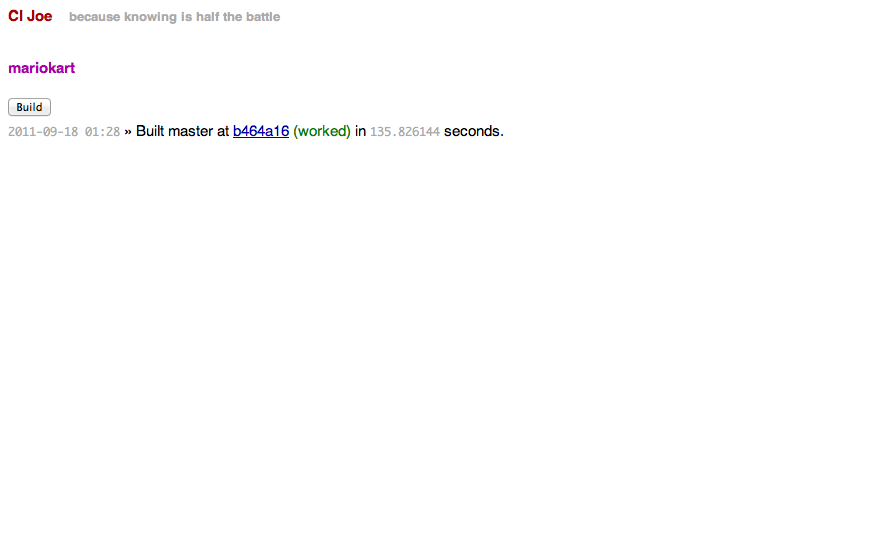
\includegraphics[width=0.45\linewidth]{images/green-full}
        }
        \only<2>{
          
\includegraphics[width=0.45\linewidth]{images/building-dashboard}
          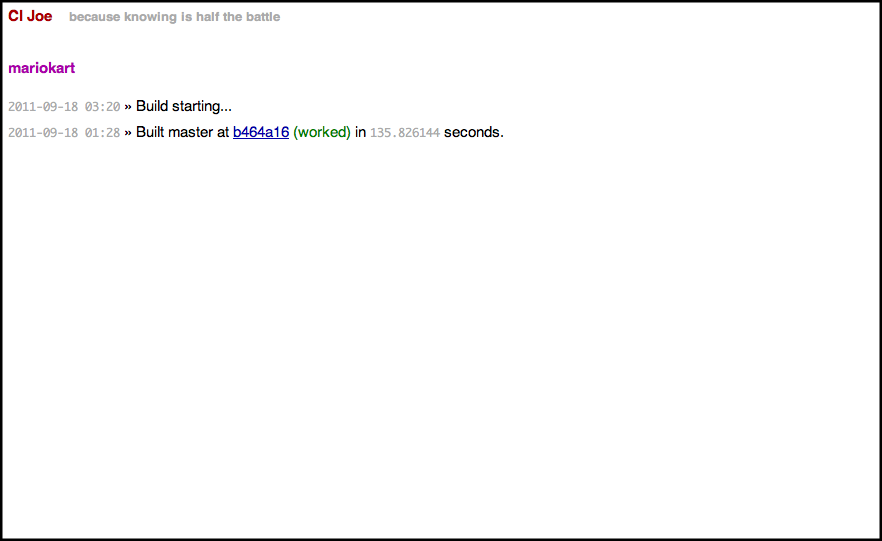
\includegraphics[width=0.45\linewidth]{images/building-full}
        }
        \only<3>{
          
\includegraphics[width=0.45\linewidth]{images/fail-dashboard}
          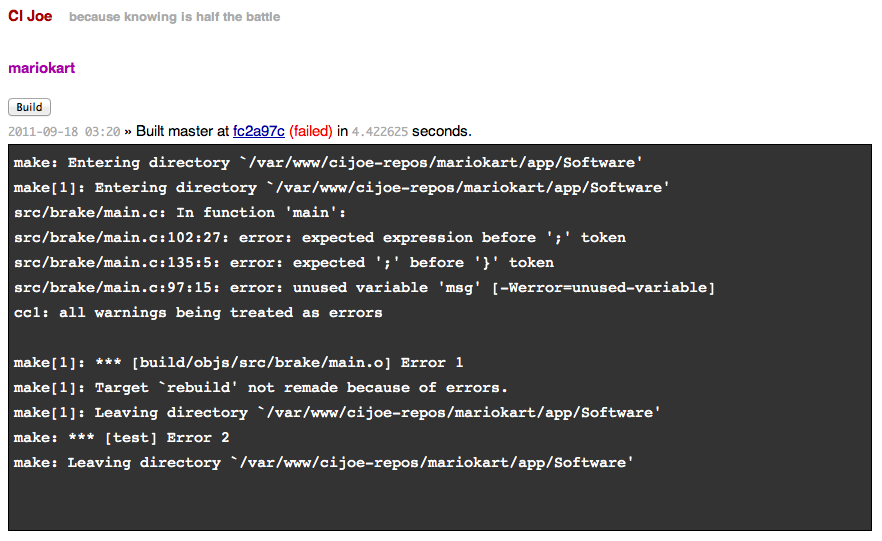
\includegraphics[width=0.45\linewidth]{images/fail-full}
        }
      \end{frame}

      \begin{frame}{Continuous Integration - Example 2}
      \end{frame}
\end{document}
